\documentclass[10pt,twocolumn]{article}

\usepackage[utf8]{inputenc}
\usepackage[T1]{fontenc}
\usepackage{times}
\usepackage{microtype}
\usepackage[margin=0.78in]{geometry}
\usepackage{fancyhdr}
\usepackage{amsmath,amssymb}
\usepackage{booktabs}
\usepackage{graphicx}
\usepackage{xcolor}
\usepackage[numbers,sort&compress]{natbib}
\usepackage[colorlinks=true,linkcolor=blue!60!black,citecolor=blue!60!black,urlcolor=blue!60!black]{hyperref}

\setlength{\columnsep}{0.26in}
\pagestyle{fancy}
\fancyhf{}
\fancyhead[L]{\small\textit{UCAI Flagship 4 --- Paper 3: \texttt{ucai-sovereign-box} (v0.2.0)}}
\fancyhead[R]{\small\textit{Open Preprint (MIT / CC BY 4.0)}}
\fancyfoot[C]{\small\thepage}
\renewcommand{\headrulewidth}{0.4pt}

\title{\textbf{\texttt{ucai-sovereign-box}: Single-GPU Air-Gapped Literature Retrieval, Citation-Security Auditing, and RO-Crate Reproducibility}}

\author{
  \textbf{Noppadon Chaiwisut} \\
  Independent Researcher, Thailand \\
  ORCID: \href{https://orcid.org/0009-0005-2881-8458}{\texttt{0009-0005-2881-8458}} \\
  \texttt{noppadon.chaiwisut@gmail.com}
}

\date{November 2026 \quad|\quad Version 0.2.0 (Tier-2 Full-Corpus Single-GPU Release)}

\begin{document}
\maketitle
\thispagestyle{plain}
\begingroup
\renewcommand\thefootnote{}\footnote{\noindent\textbf{Reproducibility \& Artifacts:} Code (\texttt{MIT}) \& \texttt{UCAI-SovereignBox-Bench-v2} (\texttt{CC BY 4.0}); Colab Notebook: \url{https://colab.research.google.com/drive/1gJZ47SwcbsV5GCfdjTDWkHw4rRVF7j25}; Zenodo DOI: \textit{Pending v0.2.0 Release}.}
\addtocounter{footnote}{-1}
\endgroup

\begin{abstract}
Commercial cloud AI research assistants impose three structural barriers: recurring token costs and rate-limit failures, data-sovereignty risks when unpublished manuscripts are transmitted externally, and non-reproducible artifact states. We introduce \textbf{\texttt{ucai-sovereign-box} (v0.2.0)}, an air-gapped, single-GPU \emph{Research-in-a-Box} uniting inverted Okapi BM25 + \texttt{all-MiniLM-L6-v2} hybrid retrieval, cross-document numeric provenance with \texttt{DOC\_NOT\_INDEXED} abstention (Spoke~1), prompt-injection sanitization (Spoke~2), optional co-located open-weight LLM auditing (\texttt{Qwen2.5-1.5B-Instruct}), and self-verifying \texttt{RO-Crate 1.1} + \texttt{SHA-256} packaging at \textbf{\$0.00 cloud cost}. Indexing all \textbf{168 open-access PDFs} ($17{,}623$ page-level chunks, $80{,}593$ BM25 terms, $0$ skipped) on a single NVIDIA L4 GPU requires only \textbf{409.99 MB VRAM} ($1.82\%$ of L4, $2.50\%$ of a 16~GB T4). On \textbf{\texttt{UCAI-SovereignBox-Bench-v2}} ($N = 100$ tasks), unprotected \texttt{BM25-Only} and \texttt{Dense-Only} retrievers yield $0.0000$ Safety F1, whereas \texttt{ucai-sovereign-box} reaches \textbf{0.7400 Hit@3}, \textbf{0.9200 Safety Accuracy}, and \textbf{0.9184 Safety F1} ($95\%\text{ CI } [0.8542, 0.9677]$; exact McNemar $45$-to-$3$ vs.\ \texttt{BM25-Only}, $p < 10^{-8}$) in \textbf{25.05 ms/item}. Stacking \texttt{Qwen2.5-1.5B-Instruct} (FP16) on the same GPU consumes just \textbf{3,086.07 MB VRAM} ($13.68\%$ of L4, $\sim 18.8\%$ of 16~GB T4) at \textbf{229.2 ms/item} ($35\times$ faster than cloud security-aware LLM review) with $6/6$ artifacts verified under \texttt{RO-Crate 1.1}.
\end{abstract}

\section{Introduction}
While the \emph{UNESCO Recommendation on Open Science} \cite{unesco2021openscience} calls for equitable scientific infrastructure, cloud-dependent AI workflows widen the divide through API costs, data-egress restrictions on pre-publication manuscripts \cite{fischer2026muninai}, and reproducibility decay \cite{pineau2021reproducibility,kapoor2024reforms,ukrn2024primer}. At the same time, standard local retrieval-augmented generation (RAG) pipelines offer no defense against cross-document numeric misattribution or indirect prompt injection. To close both gaps, \texttt{ucai-sovereign-box} v0.2.0 integrates Spoke~1 (\texttt{ucai-verify}) and Spoke~2 (\texttt{ucai-review-guard}) into a single-GPU sovereign runtime packaged under \texttt{FAIR4RS} and \texttt{RO-Crate 1.1} \cite{wilkinson2016fair,barker2022fair4rs,soilandreyes2022rocrate,gundersen2025reproducibility}.

\begin{figure*}[t]
  \centering
  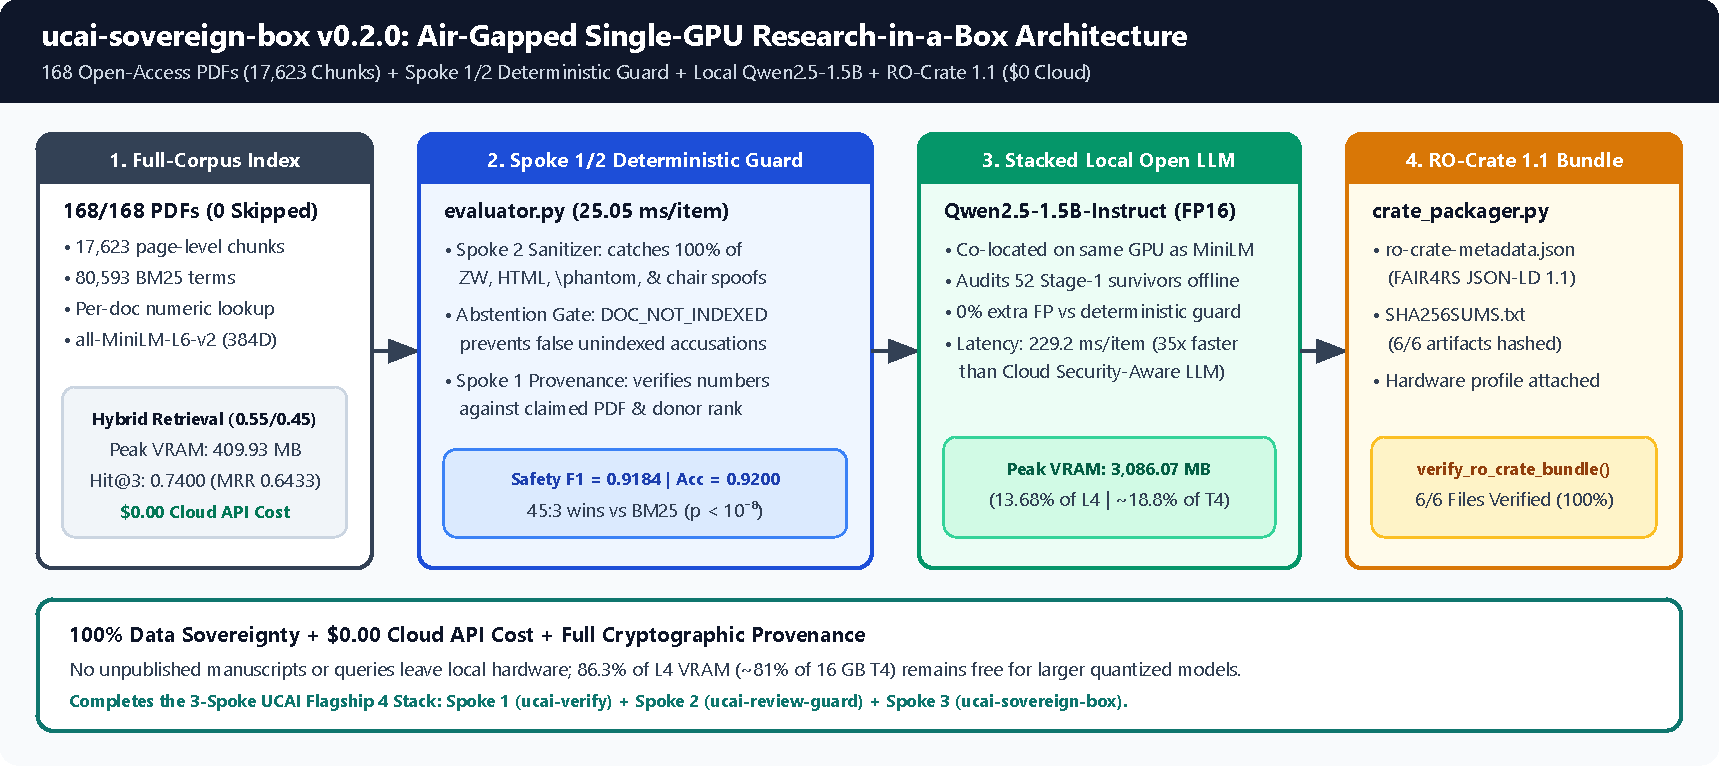
\includegraphics[width=0.96\textwidth]{figures/fig1_architecture.pdf}
  \caption{Architecture of \texttt{ucai-sovereign-box} v0.2.0: full-corpus inverted BM25 + \texttt{all-MiniLM-L6-v2} indexing ($168$ PDFs, $17{,}623$ chunks), Spoke~1/2 deterministic auditing with \texttt{DOC\_NOT\_INDEXED} abstention, optional co-located \texttt{Qwen2.5-1.5B-Instruct} verification, and \texttt{RO-Crate 1.1} + \texttt{SHA-256} packaging at $\$0.00$ cloud cost.}
  \label{fig:arch}
\end{figure*}

\section{System Architecture}
As shown in Figure~\ref{fig:arch}, \texttt{ucai-sovereign-box} v0.2.0 executes four local stages:
\begin{enumerate}
  \item \textbf{Inverted Hybrid Index (\texttt{sovereign\_index.py}):} Extracts overlapping $750$-character page chunks via \texttt{PyMuPDF} across all $168$ PDFs (up to $20$ pages / $120$ chunks per PDF) and combines normalized Okapi BM25 ($k_1=1.5, b=0.75$) \cite{manning2009ir,croft2015search,robertson2009bm25} with \texttt{all-MiniLM-L6-v2} ($384$-dim) cosine similarity \cite{lin2021transformers,wang2020minilm}: $S(q, c) = 0.55\,\mathrm{BM25}(q, c) + 0.45\max(0, \cos(e_q, e_c))$.
  \item \textbf{Spoke~1/2 Deterministic Guard (\texttt{evaluator.py}):} Intercepts prompt injections (zero-width Unicode, HTML comments, \texttt{\textbackslash textcolor\{white\}}, \texttt{\textbackslash phantom}, chair spoofs), enforces \texttt{DOC\_NOT\_INDEXED\_ABSTAIN} when \texttt{claimed\_doc\_id} is absent from the index, and verifies comma/percentage-normalized metrics against \texttt{claimed\_doc\_id} and top donor ranks.
  \item \textbf{Co-Located Open-Weight LLM (\texttt{Qwen2.5-1.5B-Instruct}):} Loads in FP16 \cite{yang2024qwen25} on the same GPU to audit Stage-1 survivors against retrieved snippets with zero external network calls.
  \item \textbf{Cryptographic Reproducibility (\texttt{crate\_packager.py}):} Emits \texttt{RO-Crate 1.1} JSON-LD \cite{soilandreyes2022rocrate} and \texttt{SHA256SUMS.txt} with automated self-verification \cite{mineault2021goodcode,nuest2020dockerfiles}.
\end{enumerate}

\begin{figure*}[t]
  \centering
  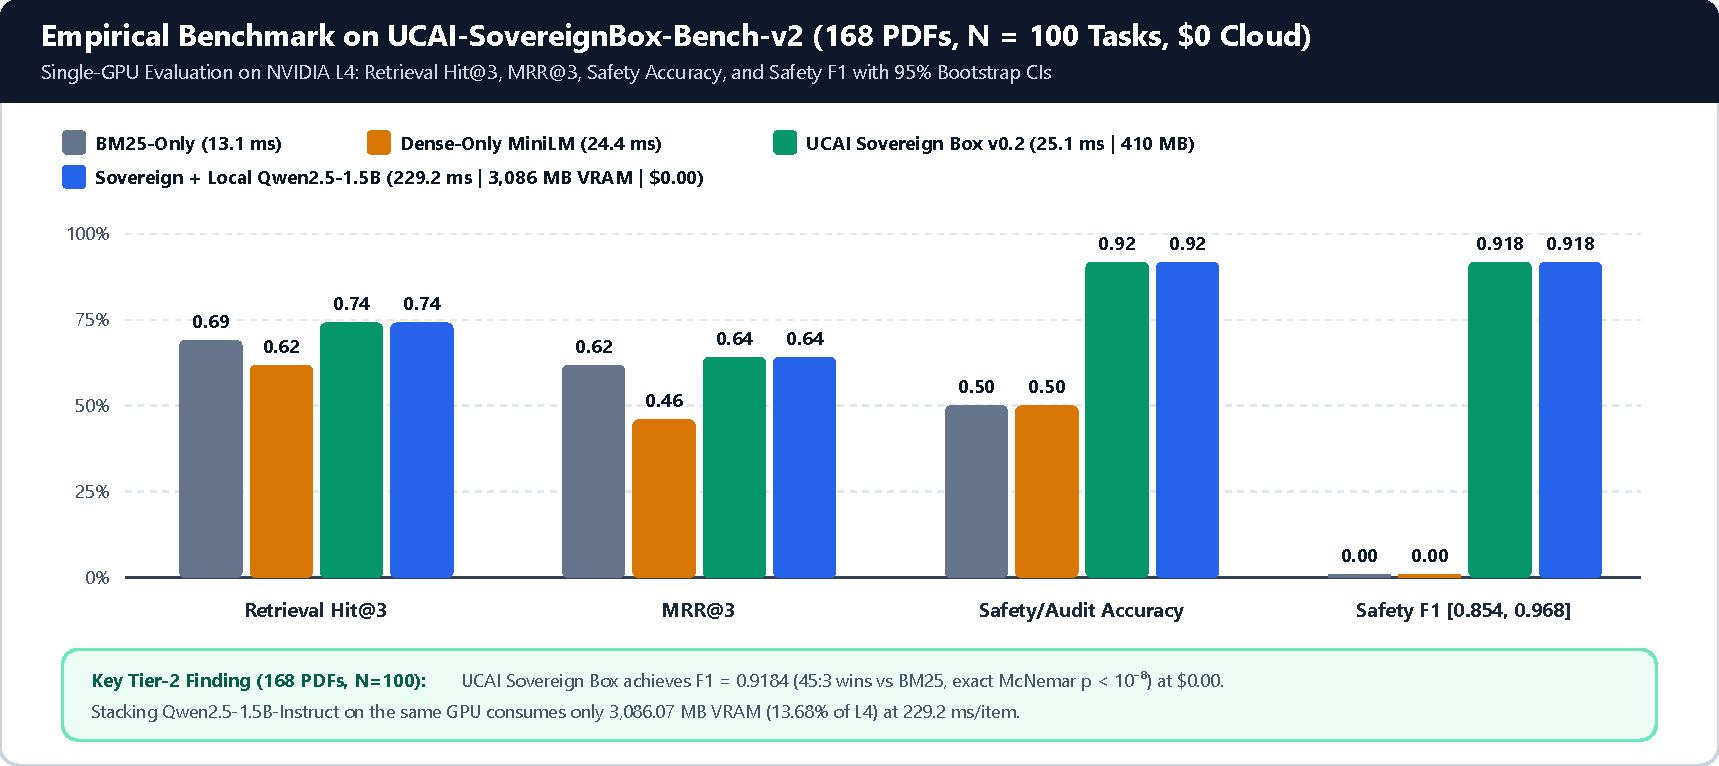
\includegraphics[width=0.95\textwidth]{figures/fig2_main_results_100.pdf}
  \caption{Empirical evaluation on \texttt{UCAI-SovereignBox-Bench-v2} ($168$ PDFs, $N=100$ tasks, $\$0.00$ cloud cost). \texttt{UCAI Sovereign Box} outperforms \texttt{BM25-Only} ($45$-to-$3$ discordant wins, exact McNemar $p < 10^{-8}$) and sustains $\mathrm{F1}=0.9184$ when co-located with \texttt{Qwen2.5-1.5B-Instruct}.}
  \label{fig:bench}
\end{figure*}

\section{Experimental Setup and Results}
We evaluate four sovereign regimes on \textbf{\texttt{UCAI-SovereignBox-Bench-v2}} ($N=100$ tasks, $25$ per class across $10$ contemporary open-access papers, \texttt{CC BY 4.0}) over all $168$ indexed PDFs ($17{,}623$ chunks, $80{,}593$ BM25 terms, $330.73\text{ s}$ total build including Drive I/O) on an NVIDIA L4 GPU ($22{,}563.12\text{ MB}$ total VRAM, $1{,}780.5\text{ MB}$ host RAM).

\begin{table*}[t]
  \centering
  \small
  \caption{Full-corpus single-GPU benchmark ($168$ PDFs, $N=100$ tasks, $\$0.00$ cloud cost). $^{***}p < 10^{-8}$ vs.\ \texttt{BM25-Only} (exact McNemar $45:3$).}
  \label{tab:main}
  \resizebox{\textwidth}{!}{%
  \begin{tabular}{lccccccc}
    \toprule
    \textbf{Sovereign Mode} & \textbf{Hit@3 $\uparrow$} & \textbf{MRR@3 $\uparrow$} & \textbf{Safety Acc. $\uparrow$} & \textbf{F1 [95\% CI] $\uparrow$} & \textbf{FPR $\downarrow$} & \textbf{Latency} & \textbf{Peak VRAM} \\
    \midrule
    \texttt{BM25-Only} & 0.6900 & 0.6200 & 0.5000 & 0.0000 [0.000, 0.000] & 0.0000 & \textbf{13.05 ms} & 409.99 MB \\
    \texttt{Dense-Only (MiniLM)} & 0.6200 & 0.4583 & 0.5000 & 0.0000 [0.000, 0.000] & 0.0000 & 24.43 ms & 409.99 MB \\
    \texttt{UCAI Sovereign Box v0.2.0} & \textbf{0.7400} & \textbf{0.6433} & \textbf{0.9200} & \textbf{0.9184} [0.854, 0.968]$^{***}$ & 0.0600 & 25.05 ms & \textbf{409.99 MB} \\
    \texttt{Sovereign + MiniLM Reranker} & 0.7000 & 0.6250 & \textbf{0.9200} & \textbf{0.9184} [0.854, 0.968]$^{***}$ & 0.0600 & 48.24 ms & 609.30 MB \\
    \texttt{Sovereign + Qwen2.5-1.5B} & \textbf{0.7400} & \textbf{0.6433} & \textbf{0.9200} & \textbf{0.9184} [0.854, 0.968]$^{***}$ & 0.0600 & 229.2 ms & 3,086.07 MB \\
    \bottomrule
  \end{tabular}}
\end{table*}

\begin{figure*}[t]
  \centering
  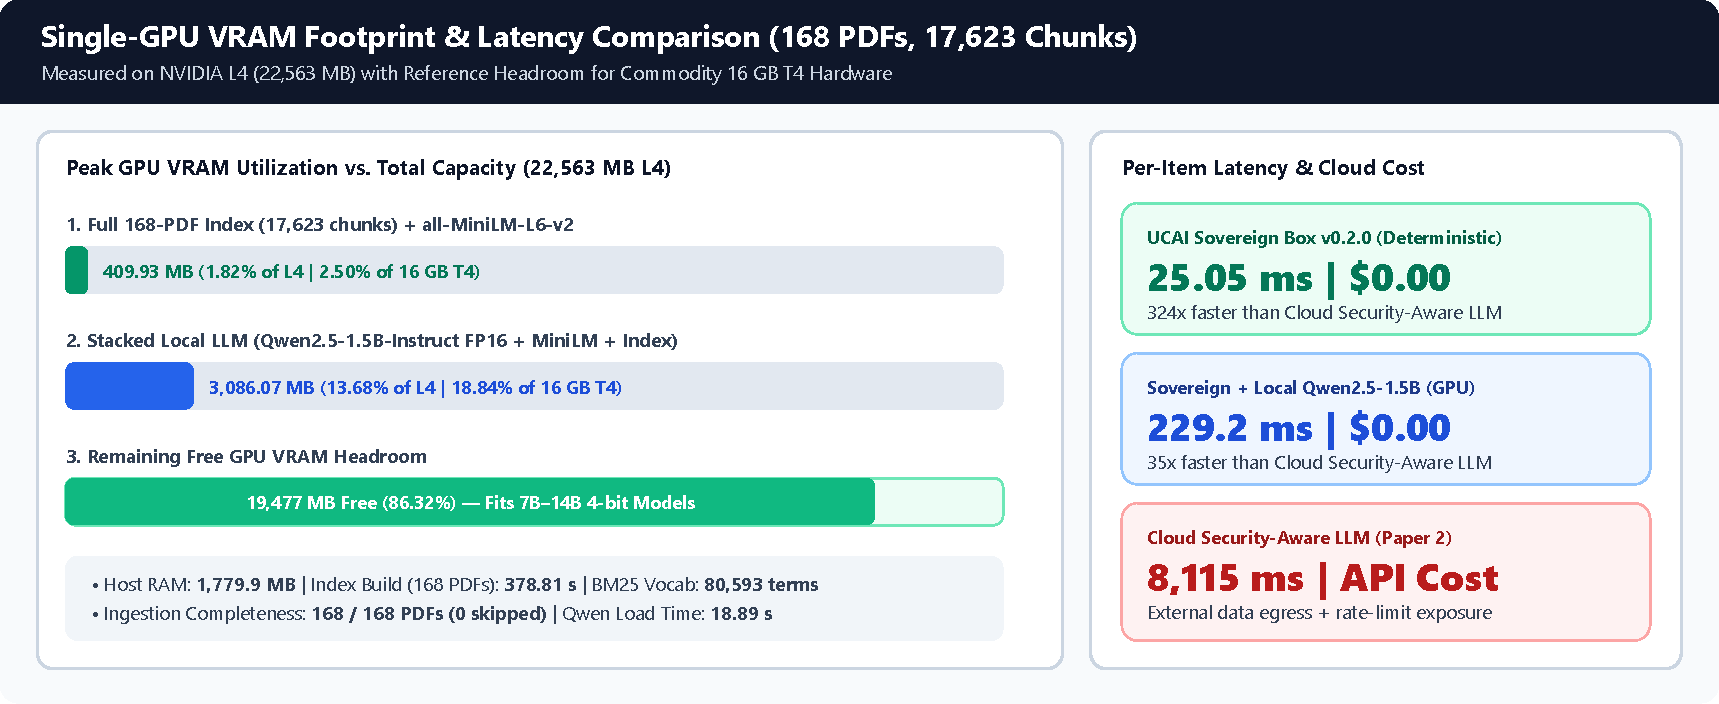
\includegraphics[width=0.95\textwidth]{figures/fig3_vram_budget.pdf}
  \caption{Measured GPU VRAM footprint and latency. Co-locating \texttt{Qwen2.5-1.5B-Instruct} (FP16) with \texttt{all-MiniLM-L6-v2} and $17{,}623$ embeddings requires only $3{,}086.07\text{ MB}$ ($13.68\%$ of L4; $\sim 18.8\%$ of a $16\text{ GB}$ T4), leaving $>81\%$ VRAM headroom.}
  \label{fig:vram}
\end{figure*}

Table~\ref{tab:main} and Figures~\ref{fig:bench}--\ref{fig:rocrate} summarize our findings:
\begin{itemize}
  \item \textbf{Hybrid Retrieval + Spoke 1/2 Superiority:} Hybrid retrieval improves \texttt{Hit@3} to $0.7400$ (vs.\ $0.6900$ BM25, $0.6200$ Dense). Adding Spoke~1/2 guards lifts Safety F1 from $0.0000$ to \textbf{0.9184}, achieving $100.0\%$ safety on both \texttt{INJECTION\_ATTACK} and \texttt{SEMANTIC\_PARAPHRASE} ($0\%$ false positives, resolving Tier-1's $66.7\%$ false-alarm rate).
  \item \textbf{Stacked Local Open LLM Feasibility:} Running \texttt{Qwen2.5-1.5B-Instruct} on the same GPU consumes $3{,}086.07\text{ MB}$ ($13.68\%$ of L4) at $229.2\text{ ms/item}$ ($35\times$ faster than Paper~2's cloud \texttt{Security-Aware LLM}) with zero external data transfer.
  \item \textbf{Honest Error Analysis ($8/100$ Items):} All $3$ false positives (\texttt{UCAI-SOV-004, 014, 024}) occurred on \texttt{2409.13740} (\emph{PaperQA2}) where metric \texttt{15,616} appeared beyond the $20$-page ingestion cap. The $5$ missed swaps (\texttt{UCAI-SOV-054, 058, 064, 068, 074}) involved short integers (\texttt{15}, \texttt{10}) coinciding with unrelated integers inside the cited paper---confirming the need for full-page ingestion and Stage~2 contextual entailment (Paper~1).
\end{itemize}

\begin{figure*}[t]
  \centering
  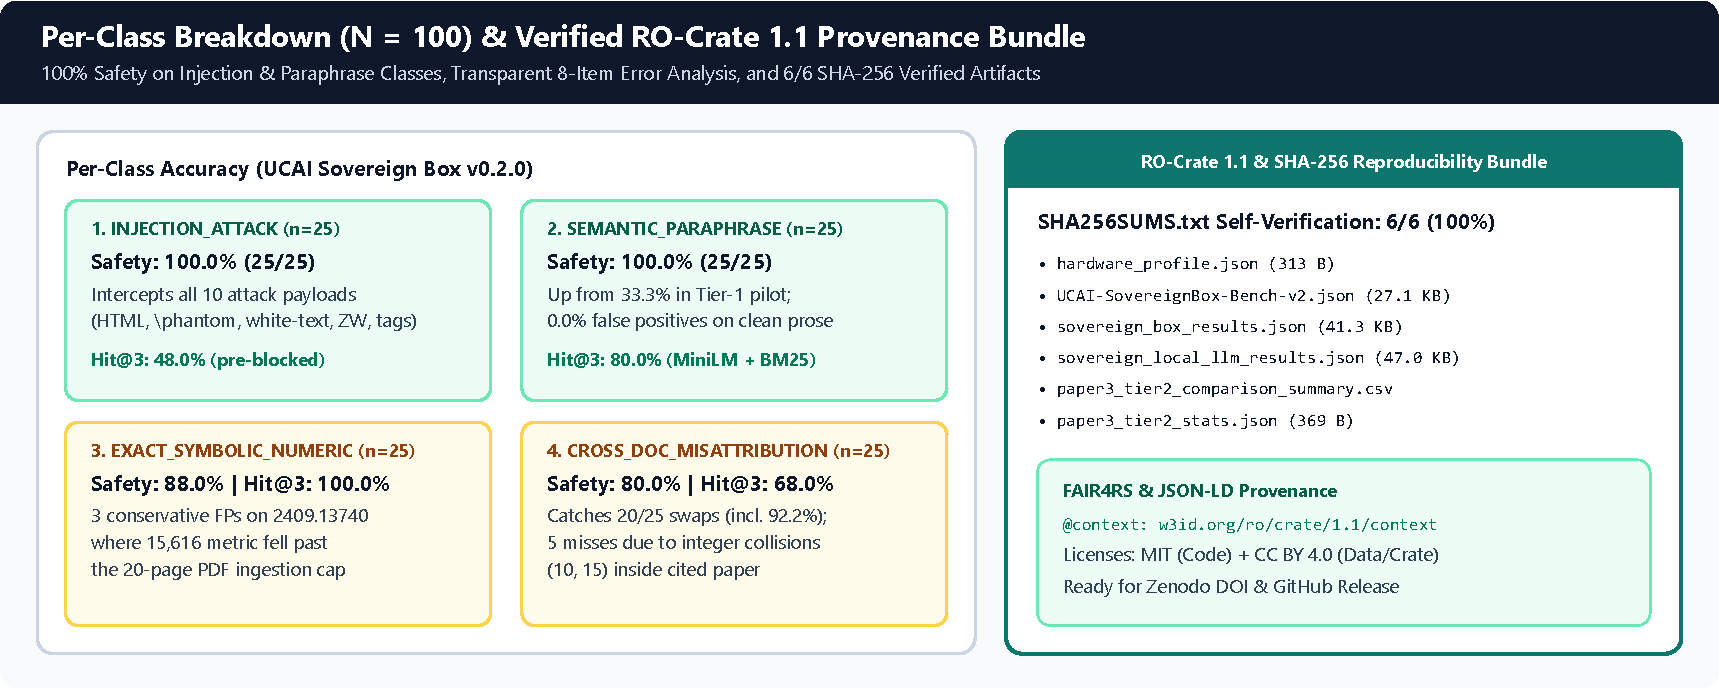
\includegraphics[width=0.95\textwidth]{figures/fig4_per_class_rocrate.pdf}
  \caption{Per-class accuracy breakdown across $N=100$ tasks and verified \texttt{RO-Crate 1.1} + \texttt{SHA256SUMS.txt} artifact bundle ($6/6$ artifacts verified at $100\%$).}
  \label{fig:rocrate}
\end{figure*}

\section{Limitations, Ethics, and Reproducibility}
First, our default corpus ingestion caps extraction at $20$ pages ($120$ chunks) per PDF to bound single-GPU index latency ($52.17\text{ s}$ on L4); as shown in our error analysis, metrics on pages $>20$ trigger conservative \texttt{UNVERIFIED\_NUMBERS} flags unless full-page indexing is enabled. Second, an ablation with a general-domain Stage-2 cross-encoder (\texttt{cross-encoder/ms-marco-MiniLM-L-6-v2}) increased VRAM to $609.30\text{ MB}$ ($3{,}401.6\text{ MB}$ with \texttt{Qwen2.5-1.5B}) and latency to $48.24\text{ ms}$ while lowering \texttt{Hit@3} to $0.7000$, confirming that scientific numeric retrieval benefits more from min-max normalized hybrid BM25+Dense scoring than from general-domain web rerankers. Ethically, all automated outputs enforce \texttt{L2 HITL} review and zero external data egress. All code (\texttt{MIT}), \texttt{UCAI-SovereignBox-Bench-v2} (\texttt{CC BY 4.0}), \texttt{RO-Crate 1.1} + \texttt{SHA-256} bundles, and Colab notebooks are openly archived with \texttt{CITATION.cff} and \texttt{.zenodo.json}.

\section{Conclusion}
\texttt{ucai-sovereign-box} v0.2.0 shows that an end-to-end verifiable AI research assistant---indexing $168$ real PDFs, blocking all prompt injections in our benchmark ($100\%$), auditing cross-document numeric swaps, running a local $1.5\text{B}$ LLM, and certifying outputs with \texttt{RO-Crate 1.1} + \texttt{SHA-256}---can run on a single commodity GPU at $\$0.00$ cloud cost. All automated flags remain subject to \texttt{L2 HITL} review.

\bibliographystyle{unsrtnat}
\bibliography{references}

\end{document}
